\chapter{MÔ HÌNH HÓA}
     \section{Mô hình hóa động học xe dò line}
          \hspace*{0.6cm}Trong chương này, nhóm thực hiện mô hình hóa robot, nhằm mục đích hiểu rõ về cấu trúc của xe, phục vụ cho việc thiết kế bộ điều khiển PID bám line cho xe.
          \newline
          \hspace*{0.6cm}Mục đích của điều khiển các động cơ DC để xe di chuyển bám line trên sa bàn trong điều kiện khá lý tưởng, với tải trọng đặt trên xe là cố định, do đó chương mô hình hóa chỉ tập trung vào xây dựng mô hình động học cho xe mà không quan tâm 
          gì đến mô hình động lực học của xe.
          \begin{figure}[H]
               \centering
               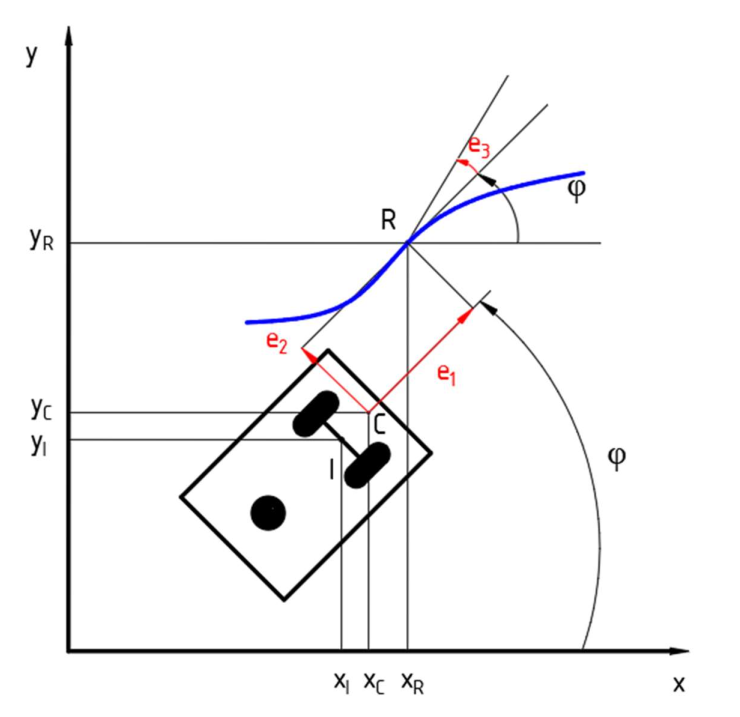
\includegraphics[width=0.7\textwidth]{pictures/chapter5/chapter5_pic1.png}
               \caption{Mô hình động học xe dò line}
               \label{kinematic_model}
          \end{figure}         
          Hình trên mô tả tọa độ các điểm cần thiết của xe trên mặt phẳng tọa độ. Trong đó
          \begin{itemize}
               \item $I(x, y)$: Trung điểm đoạn nối tâm 2 bánh chủ động.
               \item $C(x, y)$: Tâm dãy cảm biến dò line.
               \item $R(x, y)$: Tọa độ điểm tham chiếu trên đường line.
          \end{itemize}
          \hspace*{0.6cm}Phương trình động học tại $I$
          \begin{align*}
               v_{xI} &= \dot{x_I} = v \times \cos \varphi\\
               v_{yI} &= \dot{y_I} = v \times \sin \varphi\\
               \dot{\varphi_I} &= \omega
          \end{align*} 
          Đưa về dạng ma trận
          \begin{align}
               \begin{bmatrix}
                    \dot{x_I} \\
                    \dot{y_I} \\
                    \dot{\varphi_I}
                    \end{bmatrix} &= \begin{bmatrix}
                    \cos\varphi & 0 \\
                    \sin\varphi & 0 \\
                    0 & 1
                    \end{bmatrix} \begin{bmatrix}
                    v \\
                    \omega
               \end{bmatrix}
               \label{c5_e1}
          \end{align}
          \hspace*{0.6cm}Trong đó
          \begin{equation*}
               \begin{cases}
                    v = \dfrac{1}{2}(v_l + v_r) = \dfrac{r\omega_r + r\omega_l}{2} \\[0.5em]
                    \omega = \dfrac{v_r - v_l}{b} = \dfrac{r\omega_r - r\omega_l}{b}
               \end{cases}               
          \end{equation*}
          \begin{itemize}
               \item $v$: vận tốc dài của xe.
               \item $\omega$: vận tốc góc của robot.
               \item $b$: khoảng cách giữa 2 bánh xe.
          \end{itemize}
          \hspace*{0.6cm}Phương trình động học tại điểm bám line $C$
          \begin{equation}
               \begin{cases}
                    x_C = x_I + d \times \cos \varphi \\[0.5em]
                    y_C = y_I + d \times \sin \varphi \\[0.5em]
                    \varphi_C = \varphi_I = \varphi
               \end{cases}   
               \label{c5_e2}            
          \end{equation}
          \hspace*{0.6cm}Lấy đạo hàm ta được 
          \begin{equation}
               \begin{cases}
                    \dot{x_C} = \dot{x_I} - d \times \sin \varphi \dot{\varphi} \\[0.5em]
                    \dot{y_C} = \dot{y_I} + d \times \cos \varphi \dot{\varphi} \\[0.5em]
                    \dot{\varphi_C} = \dot{\varphi_I}
               \end{cases}
               \label{c5_e3}            
          \end{equation}
          \hspace*{0.6cm}Tương tự, mô hình động học tại điểm tham chiếu $R$ trên đường line
          \begin{align}
               \begin{bmatrix}
                    \dot{x_R} \\
                    \dot{y_R} \\
                    \dot{\varphi_R}
                    \end{bmatrix} &= \begin{bmatrix}
                    \cos\varphi_R & 0 \\
                    \sin\varphi_R & 0 \\
                    0 & 1
                    \end{bmatrix} \begin{bmatrix}
                    v_R \\
                    \omega_R
               \end{bmatrix}
               \label{c5_e4}
          \end{align}
          \hspace*{0.6cm}Phương trình biểu diễn sự sai lệch giữa điểm bám line $C$ và vị trí điểm tham chiếu $R$ mong muốn trên đường line
          \begin{equation}
               \begin{cases}
                    x_R - x_C = e_1 \cos \varphi - e_2 \sin \varphi \\[0.5em]
                    y_R - y_C = e_1 \sin \varphi + e_2 \cos \varphi \\[0.5em]
                    \varphi_R - \varphi_C = e_3
               \end{cases}    
               \label{c5_e5}           
          \end{equation}
          \hspace*{0.6cm}Trong đó
          \begin{itemize}
               \item $e_1$: sai số vị trí giữa điểm bám line $C$ và điểm tham chiếu $R$ theo phương vuông góc với trục hai bánh dẫn động.
               \item $e_2$: sai số vị trí giữa điểm bám line $C$ và điểm tham chiếu $R$ theo phương song song với trục hai bánh dẫn động.
               \item $e_3$: sai số góc giữa hướng của xe và hướng tiếp tuyến với sa bàn tại điểm tham chiếu $R$.
          \end{itemize}    
          \hspace*{0.6cm}Từ phương trình (\ref{c5_e5}) rút ra được hệ phương trình các sai số
          \begin{align}
               \begin{bmatrix}
                    e_1 \\
                    e_2 \\
                    e_3
                    \end{bmatrix} &= \begin{bmatrix}
                    \cos\varphi & \sin \varphi & 0 \\
                    -\sin\varphi & \cos \varphi & 0 \\
                    0 & 0 & 1
                    \end{bmatrix} \begin{bmatrix}
                    x_R - x_C \\
                    y_R - y_C \\
                    \varphi_R - \varphi_C
               \end{bmatrix}
               \label{c5_e6}
          \end{align}
          \hspace*{0.6cm}Đạo hàm 2 vế hệ (\ref{c5_e6}), khai triển và rút gọn ta thu được 
          \begin{align}
               \begin{bmatrix}
                    \dot{e_1} \\
                    \dot{e_2} \\
                    \dot{e_3}
                    \end{bmatrix} &= \begin{bmatrix}
                    v_R \cos e_3 \\
                    v_R \sin e_3 \\
                    \omega_R
                    \end{bmatrix} + \begin{bmatrix}
                    -1 & e_2 \\
                    0 & -d - e_1 \\
                    0 & -1
                    \end{bmatrix} \begin{bmatrix}
                    v_I \\
                    \omega_I
               \end{bmatrix}
               \label{c5_e7}
          \end{align}       
     \section{Tính toán thời gian lấy mẫu}
     \section{Mô hình hóa động cơ}
          \subsection{Mô hình hóa động cơ dẫn động bánh trái}    
          \subsection{Mô hình hóa động cơ dẫn động bánh phải}

     




          


